%
% File emnlp2018.tex
%
%% Based on the style files for EMNLP 2018, which were
%% Based on the style files for ACL 2018, which were
%% Based on the style files for ACL-2015, with some improvements
%%  taken from the NAACL-2016 style
%% Based on the style files for ACL-2014, which were, in turn,
%% based on ACL-2013, ACL-2012, ACL-2011, ACL-2010, ACL-IJCNLP-2009,
%% EACL-2009, IJCNLP-2008...
%% Based on the style files for EACL 2006 by 
%%e.agirre@ehu.es or Sergi.Balari@uab.es
%% and that of ACL 08 by Joakim Nivre and Noah Smith

\documentclass[11pt,a4paper]{article}
\usepackage[hyperref]{emnlp2018}
\usepackage{times}
\usepackage{url}
\usepackage{latexsym}

\usepackage[utf8]{inputenc}
\usepackage[small]{caption}
\usepackage{graphicx}

\usepackage{amsmath,amsfonts,amsthm}
\usepackage{booktabs}
\usepackage{color}
\usepackage{latexsym}
\usepackage{epsfig}
\usepackage{graphicx}
\usepackage{booktabs}
\usepackage{array}
\usepackage{multirow}
\usepackage{multicol}
\usepackage{hhline}
\usepackage{pbox}
\usepackage{threeparttable}
\usepackage{epstopdf}
\usepackage{amssymb}
\usepackage{subfigure}

\usepackage{amsmath}
\usepackage[noend]{algpseudocode}

\usepackage{diagbox}
\usepackage{paralist}
\usepackage{epsfig}
\usepackage{color}
\usepackage{ragged2e}
\usepackage[ruled,vlined,boxed,linesnumbered]{algorithm2e}
\usepackage{xcolor}
\usepackage{float}
\special{papersize=210mm,297mm}

\aclfinalcopy % Uncomment this line for the final submission
%\def\aclpaperid{***} %  Enter the acl Paper ID here

%\setlength\titlebox{5cm}
% You can expand the titlebox if you need extra space
% to show all the authors. Please do not make the titlebox
% smaller than 5cm (the original size); we will check this
% in the camera-ready version and ask you to change it back.

%\restylefloat{table}
\newcolumntype{P}[1]{>{\RaggedRight\hspace{0pt}}p{#1}}
\newcolumntype{L}[1]{>{\raggedright\let\newline\\\arraybackslash\hspace{0pt}}m{#1}}
\newcolumntype{C}[1]{>{\centering\let\newline\\\arraybackslash\hspace{0pt}}m{#1}}
\newcolumntype{R}[1]{>{\raggedleft\let\newline\\\arraybackslash\hspace{0pt}}m{#1}}

\newcommand{\ZY}[1]{\textcolor{blue}{Zhiyi: #1}}
\newcommand{\KZ}[1]{\textcolor{red}{Kenny: #1}}
\newcommand{\FX}[1]{\textcolor{cyan}{Frank: #1}}
\newcommand{\BL}[1]{\textcolor{green}{Bill: #1}}
\newcommand{\Shan}[1]{\textcolor{purple}{Shan: #1}}
\definecolor{mygray}{gray}{0.6}
\newcommand{\red}[1]{\colorbox{red}{#1}}

\newcommand{\secref}[1]{Section \ref{#1}}
\newcommand{\figref}[1]{Figure \ref{#1}}
\newcommand{\eqnref}[1]{Eq. (\ref{#1})}
\newcommand{\exref}[1]{Example \ref{#1}}
\newcommand{\algoref}[1]{Algorithm \ref{#1}}
\newcommand{\tabref}[1]{Table \ref{#1}}
\newcommand{\socvec}{SocVec}
\newcommand{\argmin}{\operatornamewithlimits{argmin}}
\newcommand{\argmax}{\operatornamewithlimits{argmax}}
\newtheorem{example}{Example}
\newtheorem{lemma}{Lemma}
\newtheorem{definition}{Definition}
\newcommand{\cut}[1]{}

\newcommand{\li}{\uline{\hspace{0.5em}}}

\newcommand{\bi}[1]{\textbf{\textit{#1}}}

\title{ExtRA: Extracting Prominent Review Aspects from Customer Feedback}

\begin{document}

% Multiple author syntax (remove the single-author syntax above and the \iffalse ... \fi here)
%\author{
	%Zhiyi Luo{\small $~^{1}$}, Shanshan Huang{\small $~^{1}$}, Frank F. Xu{\small $~^{1}$}\\
	%\textbf{ Bill Yuchen Lin{\small $~^{2}$}, Kenny Q. Zhu{\small $~^{1}$}, Hanyuan Shi{\small $~^{1}$} }\\
	%{\small $~^{1}$}Shanghai Jiao Tong University, Shanghai, China\\
	%{\small $~^{2}$}University of Southern California, Los Angelas, CA, USA\\
	%\{jessherlock,
	%huangss\_33\}@sjtu.edu.cn,
	%frankxu2004@gmail.com\\
	%yuchen.lin@usc.edu,
	%kzhu@cs.sjtu.edu.cn,
	%shihanyuan@sjtu.edu.cn \\
%}

\author{
	Zhiyi Luo, Shanshan Huang, Frank F. Xu\\
	\textbf{ Bill Yuchen Lin, Hanyuan Shi, Kenny Q. Zhu }\\
	Shanghai Jiao Tong University, Shanghai, China\\
	\{jessherlock,
	huangss\_33\}@sjtu.edu.cn,
	frankxu2004@gmail.com \\
	\{yuchenlin, shihanyuan\}@sjtu.edu.cn,
	kzhu@cs.sjtu.edu.cn \\
}

\maketitle

\begin{abstract}
Many existing systems for analyzing and summarizing customer reviews about 
products or service are based on a number of prominent review aspects. 
Conventionally, the {\em prominent review aspects} of a product type 
are determined manually. This costly approach cannot scale to large and 
cross-domain services such as Amazon.com, Taobao.com or Yelp.com where 
there are a large number of product types and
new products emerge almost everyday. 
In this paper, we propose a novel framework, for extracting the 
most prominent aspects of a given product type  from textual reviews. 
The proposed framework, ExtRA, extracts $K$ most prominent aspect terms 
or phrases which do not overlap semantically automatically without
supervision.
Extensive experiments show that ExtRA is effective and achieves the state-of-the-art performance on a dataset consisting of different product types. 
\end{abstract}

\section{Introduction}
\label{sec:intro}
Online user review is an essential part of e-commerce. 
Popular e-commerce websites feature an enormous amount of text reviews, 
especially for popular products and services. 
To improve the user experience and expedite the
shopping process, many websites provide qualitative and quantitative
analysis and summary of user reviews, which is typically organized by different 
{\em prominent review aspects}.
For instance, \figref{fig:tripadvisor} shows a short review passage from a customer on TripAdvisor.com, and the customer is also asked
to give scores on several specific aspects of 
the hotel, such as \textit{location} and \textit{cleanness}. 
With aspect-based reviews summary, potential customers can 
assess a product from various essential aspects very efficiently and directly.
Also, aspect-based review summary offers an effective 
way to group products by their prominent aspects and hence
enables quick comparison.
\begin{figure}[th!]
	\centering
	\includegraphics[width=0.7\columnwidth]{figures/tripadvisor}
	\caption{An example user review about a hotel on TripAdvisor. 
		The grades are organized by different prominent review aspects: \textit{value}, \textit{rooms}, etc. }
	\label{fig:tripadvisor}
\end{figure}                                

Existing approaches for producing such prominent aspect terms have been
largely manual work~\cite{poria2014rule,qiu2011opinion}. This is feasible for web services that only 
sell (or review) a small number of  product types of the same domain. 
For example, TripAdvisor.com only features travel-related products, 
and Cars.com only reviews automobiles, so that human annotators can provide 
appropriate aspect terms for customers based on their domain knowledge.  
While it is true that the human knowledge is useful
in characterizing a product type,
such manual approach does not scale well for 
general-purpose e-commerce platforms, such as Amazon, eBay,  
or Yelp, which feature too many product types, 
not to mention that new product and service types are emerging 
everyday.  
In these cases, manually selecting and pre-defining 
aspect terms for each type is too costly and even impractical.

Moreover, the key aspects of a product type may also change over time. 
For example, in the past, people care more about the screen 
size and signal intensity when reviewing cell phones. 
These aspects are not so much of an issue in present days. 
People instead focus on battery life and processing speed, etc.
Therefore, there is a growing need to automatically extract prominent 
aspects from user reviews.

A related but different task is \textit{aspect-based opinion 
	mining}~\cite{su2008hidden,zeng2013classification}. 
Here techniques have been developed to automatically mine
product-specific ``opinion phrases'' such as those shown in 
\figref{fig:phrases}.
In this example, the most frequently mentioned opinion phrases
about a phone model along with the mention frequency
are displayed. 
Their goal is to get the {\em fine-grained} opinion summary on
possibly overlapping aspects of a particular product.
For example, ``good looks'' and ``beautiful screen'' both comments
on the ``appearance'' aspect of the phone. However, these aspects
are implicit and can't be used in aspect-based review summarization
directly. The main disadvantage of these opinion phrases is that
their aspects differ from product to product, making it difficult to
compare the product side by side. 

\begin{figure}[th]
	\centering
	\includegraphics[width=0.75\columnwidth]{figures/phrases}
	\caption{Automatic review summarization for two mobile phones 
		on an e-commerce website}
	\label{fig:phrases}
\end{figure}


The goal of this paper is to develop an unsupervised framework 
for automatically extracting $K$ most prominent, non-overlapping 
review aspects for a given type of product from user review texts.  
Developing such an unsupervised framework is challenging for 
the following reasons: 
\begin{itemize}
	\item 
	The extracted prominent aspects not only need to cover as many customer concerns as possible but also have little semantic overlap. 
	\item The expression of user opinions is highly versatile: 
	aspect terms can be expressed either explicitly or implicitly. For example,
	the mention of ``pocket'' implies the aspect ``size''.
	\item Product reviews are information rich. A short piece of comments 
	may target multiple aspects, so topics transit quickly from sentence 
	to sentence. 
\end{itemize}

Most previous unsupervised approaches for the prominent 
aspect extraction task are variants of topic modeling 
techniques~\cite{lakkaraju2011exploiting,lin2009joint,wang2011latent}.
The main problem of such approaches 
is that they typically use only word frequency and co-occurrence information, 
and thus degrade when extracting aspects from sentences that appear
different on the surface but actually discuss similar aspects. 

Given all review text about a certain product type, our framework, ExtRA,
extracts most prominent aspect terms in four main steps: 
first it extracts potential aspect terms from text corpus by lexico-syntactic 
analysis; then it associates
the terms to synsets in WordNet and induce a subgraph that connect these
terms together; after that it ranks the aspect terms by a personalized page rank
algorithm on the sub-graph; and finally picks the top $K$ non-overlapping 
terms using the subsumption relation in the subgraph. 


The main contributions in this paper are as follows:
\begin{enumerate}
	\item We propose a novel framework for extracting prominent aspects 
	from customer review corpora (\secref{sec:method}), and provide an evaluation dataset for future work in this research area.
	\item Extensive experiments show that our unsupervised framework is effective and 
	outperforms the state-of-the-art methods by a substantial margin (\secref{sec:experiments}).
\end{enumerate}

\begin{figure*}[th!]
	\centering
	\includegraphics[width=\textwidth]{figures/framework-extra}
	\caption{Overall framework.}
	\label{fig:framework}
\end{figure*}
\section{Framework}
\label{sec:method}
In this section, we first state the \textit{review aspect extraction problem}, 
then present the workflow of our method, shown in \figref{fig:framework}.

\subsection{Problem Statement}
\label{sec:problem}
The review aspect extraction problem is given all the text reviews about
one type of product or service, extract $K$ words (or phrases), 
each of which represents a prominent and distinct review aspect. 

For instance, if the given product type is \textit{hotel}, 
we expect a successful extraction framework to extract 
$K=5$ aspect terms as follows: 
\textit{room, location, staff, breakfast, pool}.

\subsection{Aspect Candidates Extraction}
\label{sec:candidate}
Following the observation of Liu~\shortcite{hu2004mining, liu2015automated}, 
we assume that aspect terms are nouns and noun phrases.  
First, we design a set of effective syntactic rules, which can be applied across domains, to collect the aspect candidates from review texts.
We mainly use the adjectival modifier dependency relation (\emph{amod})
and the nominal subject relation (\emph{nsubj})
to extract the aspect-opinion pairs $\left\langle N, A \right\rangle$.
In addition, we leverage the conjunction relation (\emph{conj}) between 
adjectives to complement the extracted pairs. 
Formally, the extraction rules can be specified as follows:
\begin{description}
	\item[Rule 1.] If $amod(N, A)$, then extract $\left\langle N, A \right\rangle$.
	\item[Rule 2.] If $nsubj(A, N)$, then extract $\left\langle N, A \right\rangle$.
	\item[Rule 3.] If $\left\langle N, A_i \right\rangle$ and $conj(A_i, A_j)$, then extract $\left\langle N, A_j \right\rangle$.
\end{description}
In this case, $N$ indicates a noun, and $A$ (e.g. $A_i$, $A_j$) is an adjective. The dependencies (e.g. $amod(N, A)$) are expressed as \emph{rel(head, dependent)}, where \emph{rel} is the dependency relation which holds between \emph{head} and \emph{dependent}.
Note that many aspects are expressed by phrases, thus,
we extend the phrases as aspect candidates by introducing the extension rules as follows:
\begin{description}
	\item[Rule E1.] If $\left\langle N, A \right\rangle$ and $N_{-1}\_N\in P$, then use $\left\langle N_{-1}\_N, A \right\rangle$ to replace $\left\langle N, A \right\rangle$.
	\item[Rule E2.] If $\left\langle N, A \right\rangle$ and $N\_N_{+1}\in P$, then use $\left\langle N\_N_{+1}, A \right\rangle$ to replace $\left\langle N, A \right\rangle$.
\end{description}
where $N_{-1}$ and $N_{+1}$ denotes the noun word,
and the subscript represents displacement to $N$ in the 
sentence. 
We use AutoPhrase~\cite{liu2017phrase} to extract a set of
phrases $P$ with high coherence.
Then we use $P$ to filter
out the incoherent phrases so as to obtain the high-quality phrases as aspect candidates.
The example in \figref{fig:framework} (Stage 1) demonstrates the extraction process. 
For example, we extract the pair $\langle$ \emph{great}, \emph{zoom\_lens }$\rangle$ from sentence (1) by applying
\emph{Rule 1} and \emph{Rule E1}.
Similarly, the extraction rules match
$\langle$ \emph{slower}, \emph{autofocus} $\rangle$,
$\langle$ \emph{noisy}, \emph{shutter} $\rangle$,
$\langle$ \emph{cheap}, \emph{lens\_cover} $\rangle$ in 
sentence (2) and 
$\langle$ \emph{quick}, \emph{shutter} $\rangle$, $\langle$ \emph{quiet}, \emph{shutter} $\rangle$ in sentence (3) as potential aspect-opinion pairs.
After extracting such pairs from the text reviews, 
we sort them by the number of occurrences,
and extract the nouns and noun phrases in the top pairs
as aspect candidates, assuming that
the most prominent aspects are subsumed by those candidates 
terms. 


\subsection{Aspect Taxonomy Construction}
\label{sec:taxonomy}
The aspect candidates extracted in the last stage come with the counts 
modified by adjectives. We can directly use such raw counts to rank 
the aspect candidates. This is one of the baseline models in 
our experiments.
However, such ranking usually suffers from the aspect overlapping problem
which obviously violates the principle of pursuing both coverage and 
distinctiveness of prominent aspects.
For example, given the number of prominent aspects 
$K$ as 5,
we can extract both of `location` and `place` aspects from
the hotel reviews. 
In order to solve this problem, we construct an aspect taxonomy 
to obtain such overlapping information between aspect candidates by
leveraging the WordNet ontology. 

\subsubsection{WordNet Synset Matching}
\label{sec:match}
First, we need to match our aspect candidates onto WordNet synsets.
The accuracy of synset matching is very important for our 
aspect taxonomy construction.
This is actually a classical word sense disambiguation (WSD) problem.
Our initial attempt is to use a Python WSD tool~\cite{pywsd14}.
For each aspect candidate, we take it as the target and 
randomly sample a bunch of sentences that contain this target. 
We use the extended word sense disambiguation algorithm~\cite{banerjee2003extended} 
in this tool. We count the total occurrences for each noun 
sense (synset) of the candidate and match the candidate to the most frequent
synset.  However, such a method is not good enough for our problem,
as shown in the results later.
It only considers the local context information within the review sentence. 
Whats more, the review sentences are usually very 
short and colloquial, which makes it 
more difficult to match properly by a common WSD algorithm.
Therefore, it is critical to construct more reliable contexts for 
aspect candidate matching. 

To achieve this goal, we cluster
the aspect candidates with similar semantics together.
Then, for each aspect candidate, 
we take the other candidates within the same cluster
as its context for later disambiguation.
As shown in the first step of stage 2 in \figref{fig:framework}, 
the semantic similar aspect candidates such as 
{\em lens, lens\_cover, zoom\_lens, exposure and shutter}
are clustered together.
For example, we can disambiguate the sense of \emph{shutter} by 
leveraging {\em lens, lens\_cover, zoom\_lens, and exposure}.
We observed that our aspect candidates can be fine-grain 
clustered with a two-stage k-means clustering 
method,\footnote{The implementation details are in \secref{sec:base}.}
which generates the better context for the 
aspect candidates.  More specifically, for a particular aspect candidate $a_t$ 
from the cluster $C = \lbrace a_1, a_2, ..., a_t, ..., a_n \rbrace$, 
we calculate the context vector of $a_t$ as:
\begin{equation}
c(a_t) = \sum_{i=1, i\neq t}^{n} E(a_i),
\end{equation}
where $c(a_t)$ denotes the context vector of $a_t$, 
and $E(a_i)$ represents the embedding of $a_i$.
The set of candidate synsets 
$S(a_t) = \lbrace s^t_1, s^t_2, ..., s^t_m \rbrace$ 
consists of the noun senses (e.g. $s^t_i$) of $a_t$  from WordNet.
Each sense $s^t_i$ is associated with a \emph{gloss} $g^t_i$
(i.e. a brief definition of $s^t_i$) which 
covers the semantics of the sense.
Therefore, we encode $s^t_i$ as the summation
of the word vectors in $g^t_i$:
\begin{equation}
\label{gloss_vec}
v(s^t_i) = \sum_{j=1}^{q} E(w^{t,i}_j),
\end{equation}
$W(g^t_i)$ is the sequence of words in $g^t_i$, i.e., 
$W(g^t_i) = \lbrack w^{t,i}_1, w^{t,i}_2, ..., w^{t,i}_q \rbrack$.
For each candidate sense $s^t_i$ of 
the aspect candidate $a_t$,
we calculate the cosine semantic similarity
between $v(s^t_i)$ and $c(a_t)$, and
match $a_t$ to the most similar $s^t_i$.

\subsubsection{Aspect Taxonomy Extraction from WordNet}
\label{wordnet}
In order to construct the aspect taxonomy from WordNet,
we first extract the hypernym paths for every matched synsets
in the previous step.
By definition, 
a hypernym path $p$ of synset $s$ is the is-a relation path 
from $s$ to the root synset (i.e. entity.n.01 for nouns).
We extract the hypernym paths for each matched synset $s_i$ 
in the WordNet ontology.
Next, we scan over all the collected paths once to construct
the aspect taxonomy which is a directed acyclic graph (DAG).
In $p$, $s_1$ is the synset matched from our potential aspects,
and $s_{i+1}$ is the hypernym of $s_i$.
As shown in step 2 of Stage 2 in \figref{fig:framework},
we match the aspect candidate \emph{shutter} to \emph{shutter.n.01}.
The only one hypernym path of \emph{shutter.n.01} is 
\emph{[shutter.n.01, optical\_device.n.01, device.n.01, ..., entity.n.01]}.

However, the matched synset usually has multiple hypernym paths 
in WordNet. 
We use the following strategy to compact and minimize the
aspect taxonomy:
\begin{itemize}
	\item Among all the paths from an aspect candidate $s_1$, 
	we will keep those paths that contain more than 1 aspect candidates, 
	unless there's only one path from $s_1$.
	If all paths contain only 1 aspect candidate $s_1$ each, we will keep all of them.
	
	\item To further optimize the taxonomy structure, we 
	induce a minimum subgraph from the original taxonomy using
	a heuristic algorithm~\cite{kou1981fast}. Such a subgraph
	satisfies the following conditions: 
	1) it contains all the nodes matched from aspect candidates;
	2) the total number of nodes in the graph is minimal.
	Consequently, the induced graph is a weakly connected DAG.
\end{itemize}
After acquiring the aspect taxonomy for the given product or service,
we can now tell if two aspects are semantically overlapped or not. 

\subsection{Aspect Ranking}
\label{sec:rank}
In this section, we propose a novel
method based on personalized page rank 
to compute the overall rank values
for the potential aspects by leveraging the aspect taxonomy.

Let the aspect taxonomy be a graph $G=(V, E)$.
Each node $v\in V$ is a synset in the aspect taxonomy and encoded 
as a vector by instantiating $E$ as Glove embeddings in \eqref{gloss_vec} .
Each edge $e = \langle u, v \rangle$ carries a weight which is
the semantic similarity between the nodes $u$ and $v$,
computed using cosine similarity.

Next, we perform the random walks on our constructed
aspect taxonomy.
The propagation starts from candidate aspect nodes in the 
aspect taxonomy, which are called {\em seeds} here.
The rank values (aspect importance) of all nodes are:
\begin{equation}
x_t = (1-\alpha)*Ax_{t-1} + \alpha*E \text{,}
\label{eq:ppr}
\end{equation}
where $t$ is the time step in random walk process.
In the initial state $E$(i.e. $x_0$), the aspect importance only distributes on the seeds ($v\in V_b$). 
$E_i$ is the i-th dimension of $E$, indicating
the portion of aspect importance on node $s_i$ 
at time step 0.
$E$ is calculated as follows:
\begin{equation}
E_i = 
\begin{cases}
\frac{f(le(s_i))}{\sum_{j=1}^{n} f(le(s_j))} &  \text{, if $s_i$ is a seed} \\
0 &  \text{, otherwise,}
\end{cases}
\end{equation}
where $n$ is the number of nodes in the graph,
$s_i$ is the synset node,
$le(s_i)$ denotes the lemma form of $s_i$,
and $f(le(s_i))$ represents the frequency that 
$le(s_i)$ is modified by adjectives.

The aspect importance is updated using the transition probabilities matrix 
$A$ which are the normalized weights on the edges of the taxonomy. 
$\alpha$ is the teleport probability, which is 
the probability of returning to the initial distribution
at each time step. 
$\alpha$ determines the distance of propagation of the taxonomy. 

\subsection{Aspect Generation}
\label{sec:generation}
Finally, we generate the prominent aspects 
using the rank values of the aspects as well as the is-a relations
in the aspect taxonomy.

We sort $le(s_i)$ in decreasing order by their rank values.
We essentially take the top aspects from the sorted list.
However there might be two types of overlapping that we need to
avoid:
i) duplicate: different synset nodes may map to the same aspects, 
i.e., $le(s_i) = le(s_j), s_i \neq s_j$ ( aspects);
ii) taxonomy overlap: the later aspect in the list is the 
hypernym or hyponym of the one of previous aspects.
To this end, we just skip overlapped aspect, and move along the list
until we generate $K$ non-overlapping prominent aspects from the list.

% experiments
\section{Experiments}
\label{sec:experiments}
We compare the ExtRA framework with 
multiple strong baselines on extracting aspect terms from user reviews. 
We first introduce the dataset and the competing models, then
show the quantitative evaluation as well as qualitative analysis for
different models.

\subsection{Dataset}
\label{sec:dataset}
We use the customer review corpora of 6 kinds of product and service
\footnote{The data is available from
	\url{http://times.cs.uiuc.edu/~wang296/Data/} and 
	\url{https://www.yelp.com/dataset}} collected from popular websites, 
including Amazon, TripAdvisor and Yelp. 
The number of hotel reviews \cite{Wang2011LearningOD} in the original
corpus is huge. 
Therefore, we randomly sample 20\% of the reviews to perform our experiments.
The statistics of the corpora are shown in~\tabref{table:dataset}.

\begin{table}[th!]
	\small
	\centering
	%\vspace{-0.3cm}
	\caption{Dataset statistics.} 
	\label{table:dataset}
	%\vspace{-0.2cm}
	\begin{tabular}{|c|c|c|}
		\hline
		\textbf{Product type} & \textbf{Source} & \textbf{\#Reviews} \\ \hline \hline
		hotel        & TripAdvisor & 3,155,765   \\\hline
		mobile phone & Amazon & 185,980  \\\hline
		mp3 player   & Amazon & 30,996   \\\hline
		laptop       & Amazon & 40,744   \\\hline
		cameras & Amazon & 471,113  \\\hline
		restaurant   & Yelp & 269,000   \\\hline
	\end{tabular}
	%\vspace{-0.2cm}
\end{table}

Existing published aspect extraction datasets ~\cite{hu2004mining,popescu2007extracting,pavlopoulos2014aspect,ding2008holistic} 
include only fine-grained aspects from reviews,
which are not suitable for evaluating the performance of 
prominent aspects extraction. 
Therefore, we build a new evaluation dataset particularly 
for this task.
Following the previous work 
~\cite{ganu2009beyond,brody2010unsupervised,zhao2010jointly,wang2015sentiment} as well as
the popular commercial websites (e.g. TripAdvisor), 
which most manually labeled 3-6 prominent aspects for
rating, we set $K$ as five.
Therefore,  
we ask each annotator who are familiar with the domain 
to give 5 aspect terms which they think are most important
for each category. We have five annotators in total.
\footnote{The 
	complete labeled set of ExtRA is released at \url{http://adapt.seiee.sjtu.edu.cn/extra/}.
}
One prominent aspect can be expressed by different terms.
Thus, it is difficult to achieve a satisfied inner-agreement.
We propose two evaluation methods, especially the 
soft accuracy in \secref{sec:quaneval} to compensate this problem.
To acquire a relatively higher inner-agreement, 
we educate the annotators with top 100 frequent aspect candidates
as hints. Though, they are not required to pick up labels from 
the candidates.
The inter-annotator agreement of each
product type shown in \tabref{agreement} is computed as the average jaccard similarity between every two annotators.

\subsection{Baselines and ExtRA}
\label{sec:base}
We introduce three topic modeling based baselines for the task.
These are \textbf{LDA}~\cite{Blei2003LatentDA}, 
\textbf{BTM}~\cite{cheng2014btm} and  
\textbf{MG-LDA}~\cite{titov2008modeling}. MG-LDA is a strong
baseline which attempts to capture multi-grain topics (i.e. global \& local), where the local topics correspond to the rateable prominent aspects.
We treat each review as a document and perform those models
to extract $K$ topics.
Then, we select most probable words in 
each topic as our extracted aspect terms. 
To prevent extracting the same aspects ($w$) from different topics, 
we only keep $w$ for the topic $t$ with the highest 
probability $p(w|t)$ value, then re-select aspects for the other 
topics until we get $K$ different aspects. 
For fair comparison among different models, the number of 
target aspects $K$ is set as 5. The hyper-parameter of 
MG-LDA (global topics) is set to 30 with fine-tuning.

Another syntactic rule-based baseline model 
\textbf{AmodExt} is from the first stage of our framework. 
After extracting the aspect candidates using
\emph{amod-rule} in \secref{sec:candidate}, 
we sort the aspect candidates by 
their counts of extracted occurrences. 
Then select the top $K$ 
candidates as the prominent aspects.

\textbf{ABAE}~\cite{DBLP:conf/acl/HeLND17}  is a neural based model that can
to infer $K$ aspect types. 
Each \emph{aspect type} is a ranked list of representative words.
To generate $K$ prominent aspects, 
we first infer $K$ aspect types using \emph{ABAE}, 
then select the most representative word from each
aspect type. 

For \textbf{ExtRA}, in the taxonomy construction stage, 
we use a two-stage K-means clustering method for synset matching task, 
and the cluster number
is auto-tuned using silhouette score~\cite{rousseeuw1987silhouettes}.
We use SkipGram~\cite{miko} model to train the embeddings
on review texts for k-means clustering. 
We set the dimension of the embeddings as 100
and run 64 epochs for each product corpora. 
In the aspect ranking stage, 
we empirically set the teleport probability $\alpha$
as $0.5$ which indicates that the expected walk-length
from the seeds is $\frac{1}{\alpha}=2$.


% eval
\subsection{Evaluation}
\label{sec:endeval}
In this section, we compare ExtRA with five baseline models 
both quantitatively and qualitatively.

\subsubsection{Quantitative Evaluation}
\label{sec:quaneval}
First, we perform two experiments to justify our aspect taxonomy construction stage:
\begin{itemize}
	\item 
	To justify the synset matching step,
	we compare our proposed cluster method with classical WSD algorithm (Lesk) on matching accuracy.
	We manually label 100 sampled synset nodes for each category.
	The synset matching accuracies are shown in 
	\tabref{synsetmatching}.
	We can see that our clustering method is effective 
	for the synset matching task.
	\item 
	We induce the aspect taxonomy using a heuristic algorithm to obtain
	more compact and aspect-oriented subgraph. 
	We show the size of aspect taxonomy induced before and after 
	taxonomy minimization in \figref{fig:size}.
\end{itemize}

\begin{table*}[]
	\small
	%\scriptsize
	\centering
	\caption{WordNet Synset matching accuracies}
	\label{synsetmatching}
	\begin{tabular}{|c|c|c|c|c|c|c|}
		\hline
		& hotel & mp3 & cameras & \begin{tabular}[c]{@{}l@{}}mobile\\ phone\end{tabular} & laptop & restaurant \\\hline\hline
		LESK    & 0.71  & 0.59 & 0.62    & 0.64     & 0.53   & 0.65          \\\hline
		Cluster & \textbf{0.86}  & \textbf{0.83} & \textbf{0.74}    & \textbf{0.80}                                                   & \textbf{0.78}   & \textbf{0.69}         \\\hline
	\end{tabular}
\end{table*}

\begin{table*}[!h]
	%\scriptsize
	\small
	\centering
	%	\vspace{-0.3cm}
	\caption{Inner-annotator agreements}
	\label{agreement}
	\begin{tabular}{|c|c|c|c|c|c|c|}
		\hline
		& hotel & mp3 & cameras & \begin{tabular}[c]{@{}l@{}}mobile\\phone\end{tabular} & laptop & restaurant \\\hline\hline
		Jaccard    & 0.470  & 0.554 & 0.304    & 0.440     & 0.271   & 0.671          \\\hline
	\end{tabular}
\end{table*}



\begin{figure*}[!ht]%
	\centering
	\subfigure{%
	\label{fig:first}%
	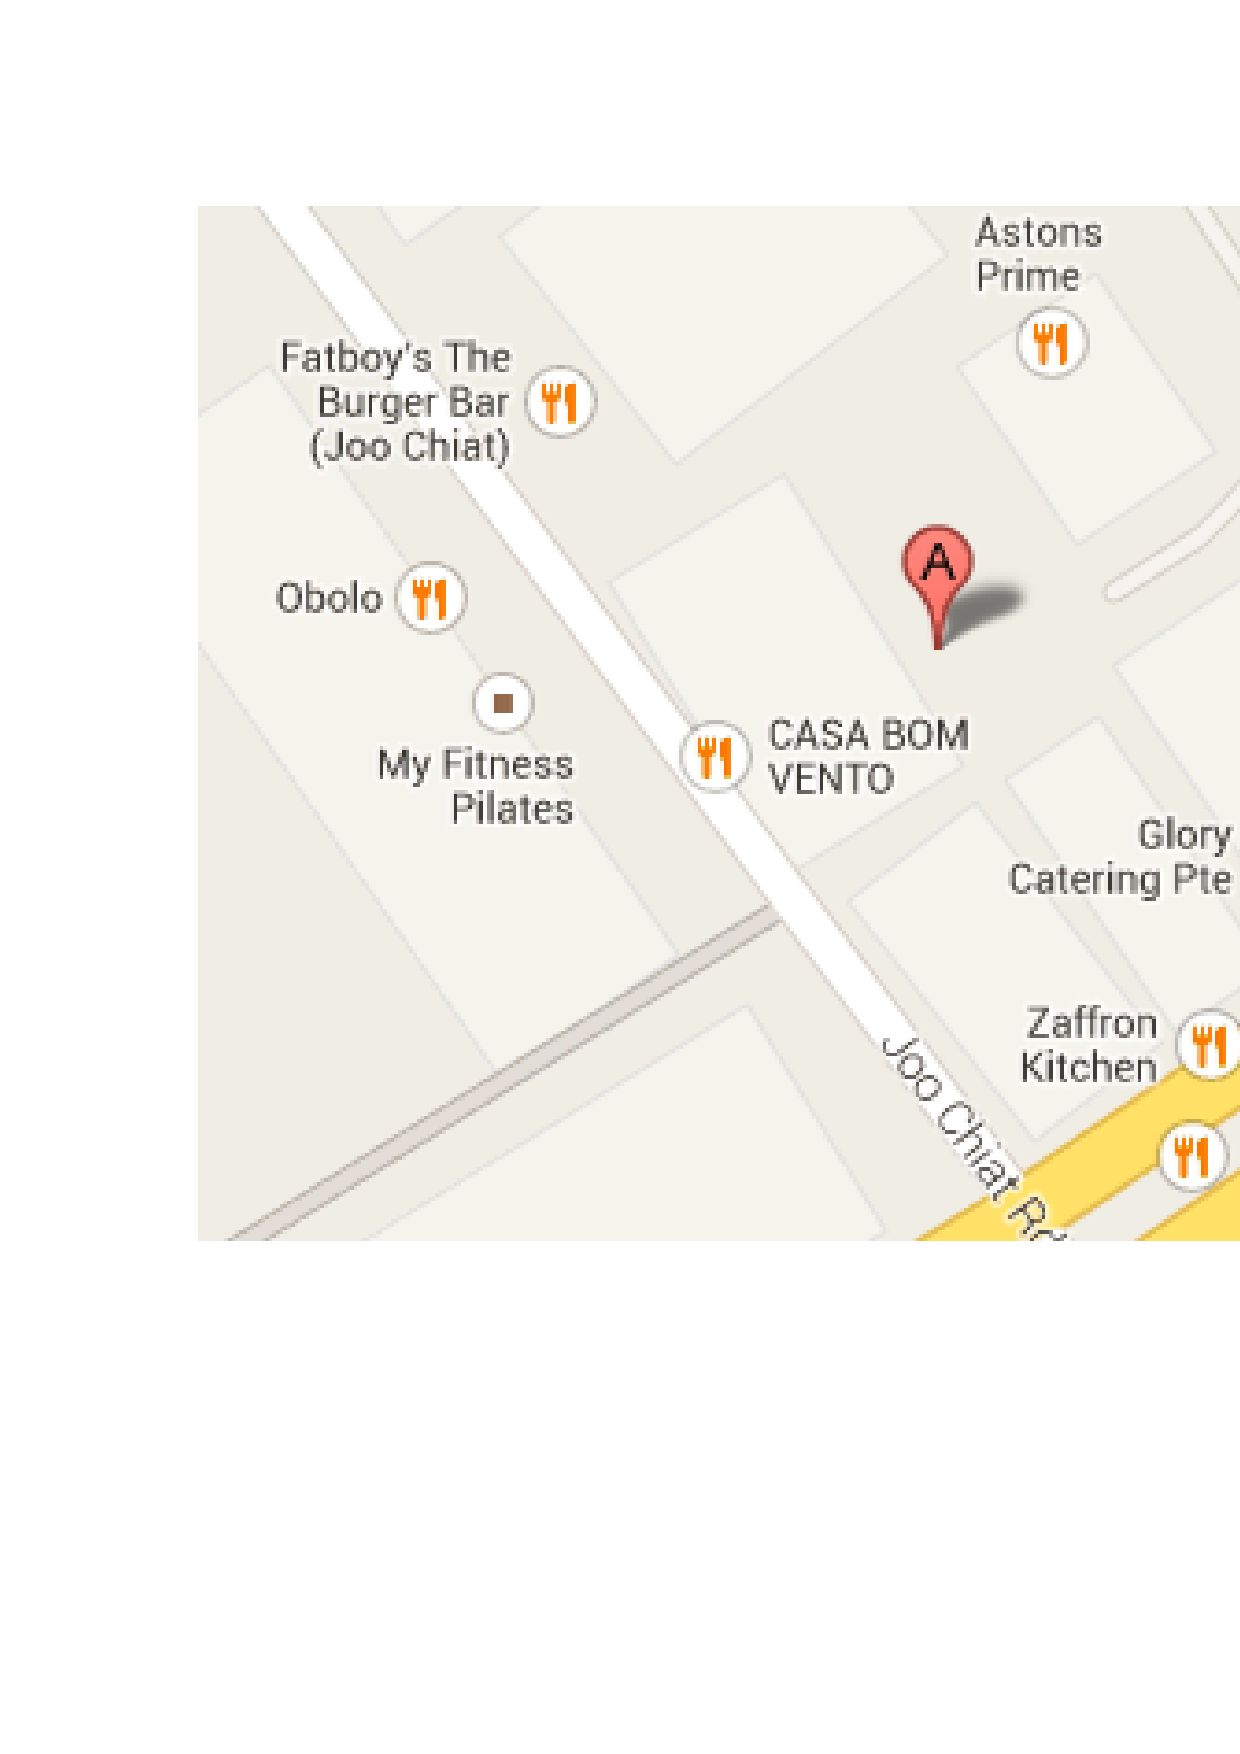
\includegraphics[width=0.8\columnwidth]{figures/1.pdf}}%
	\qquad
	\subfigure{%
	\label{fig:second}%
	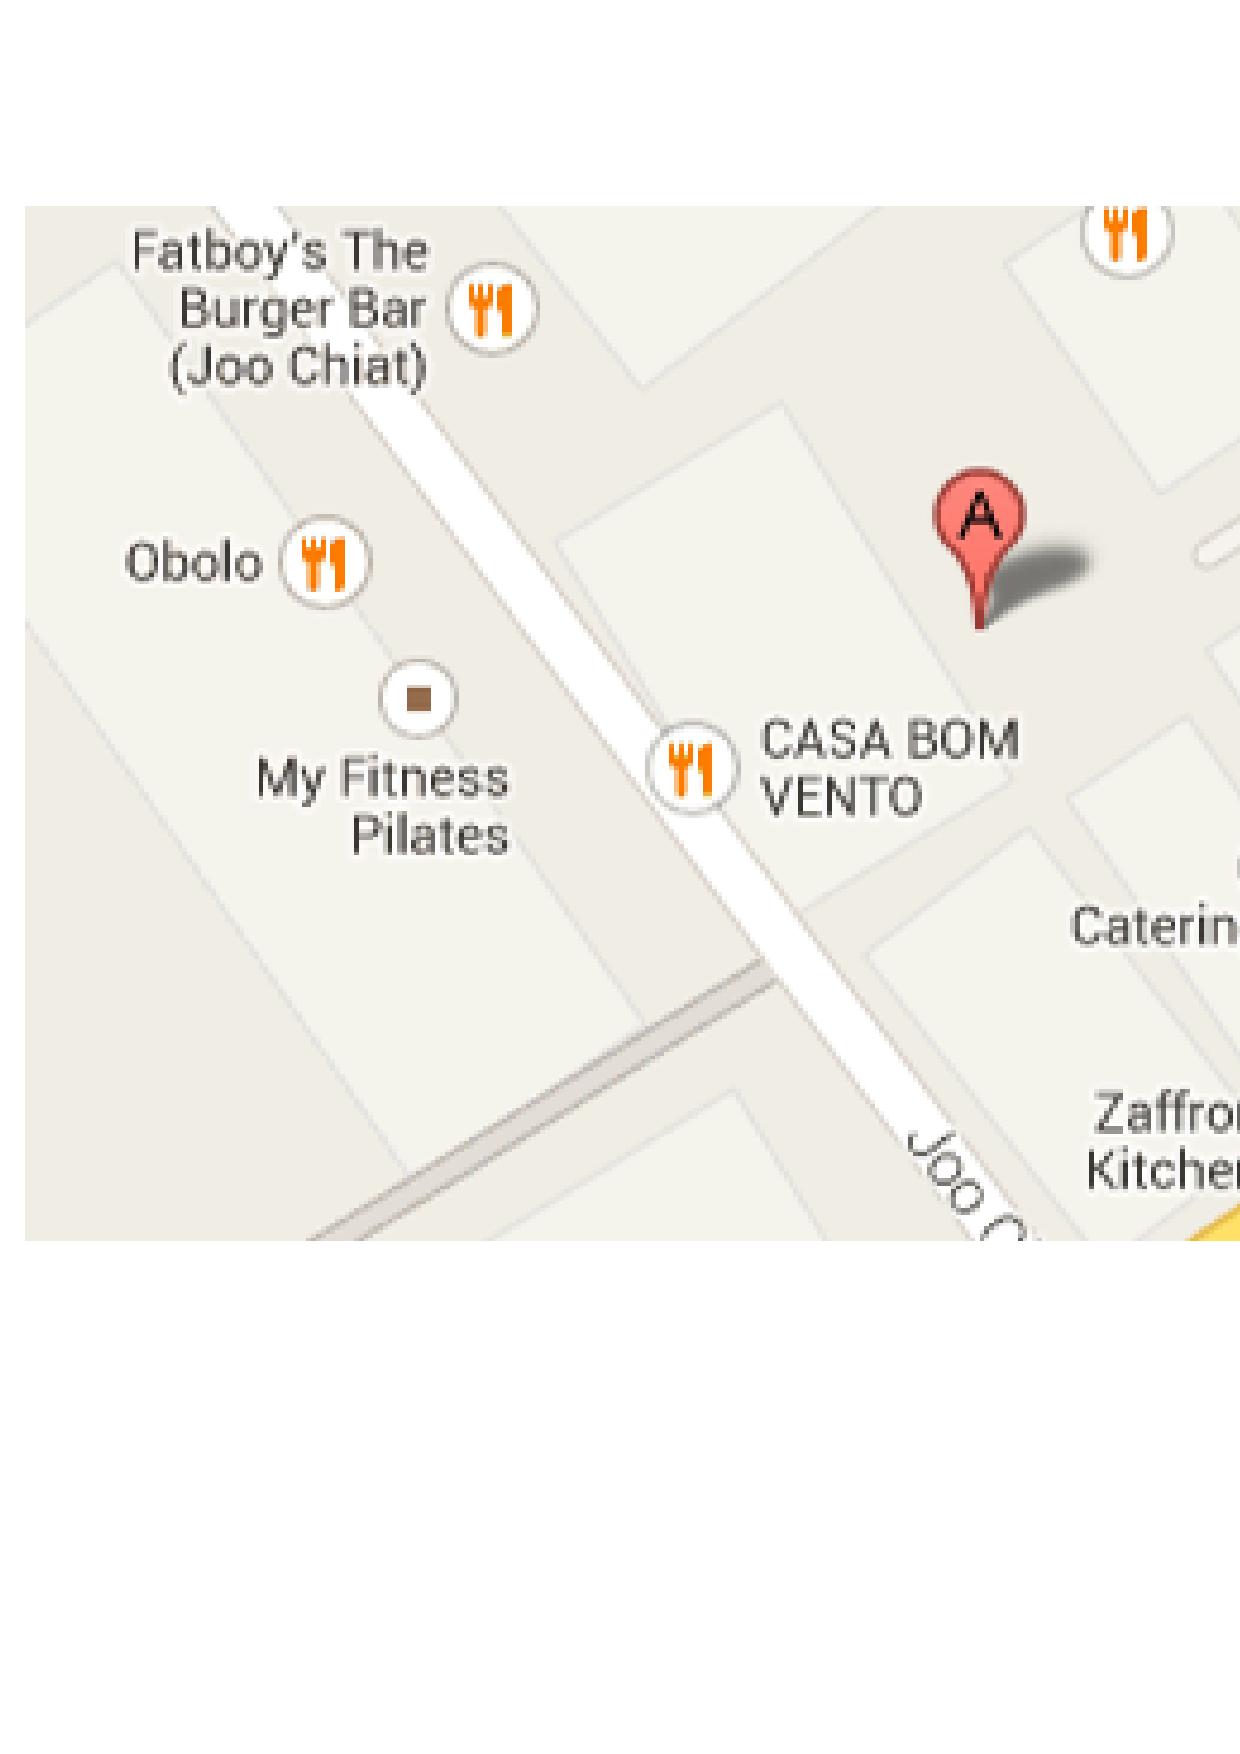
\includegraphics[width=0.8\columnwidth]{figures/2.pdf}}%
	\caption{Statistics of induced aspect taxonomy before and after taxonomy minimization}
	\label{fig:size}
\end{figure*}


Next, we evaluate our model as well as above baselines on the evaluation dataset described above.
We did not remove the duplicate aspect labels for the qualitative evaluation, 
since the repeated aspects are assume to be better.
For a given category, we first calculate the percentage of the 25 labels that exactly match one of the 5 aspect terms generated by the model 
as the \textit{hard accuracy} 
of the model. 
Formally, $Aspects(m) = [a_1, a_2, a_3, a_4, a_5]$ denotes 
the five prominent aspects generated from model $m$ for 
the given category.
$L = [l_1, l_2, ..., l_{25}]$ are the 25 golden aspect terms,
where $L^{(h)}= [l_{5h-4}, ..., l_{5h}]$ are from the $h$-th human annotator.
The hard accuracy is defined as:
\begin{equation}
hacc(m) = \frac{\sum_{i=1}^{25}{hit(Aspects(m), l_i)}}{25}
\end{equation}
\begin{equation}
hit(Aspects(m), l_i) = 
\begin{cases}
1, & l_i \in Aspects(m) \\
0, & \text{otherwise, }
\end{cases}
\end{equation}

However, counting the number of exact matches 
makes the accuracy score discrete and coarse. 
Besides, it penalizes aspect terms that don't match the label
but actually have similar meanings.
To remedy this, we propose the \emph{soft accuracy}  evaluation measure.
For each set of five golden labels from 
$h$-th annotator, we first align each generated aspect $a_k \in Aspects(m)$
with one golden aspect $l_j \in L^{(h)}$ (i.e. $align^{(h)}(a_{k})=l_{j}$). 
We align the exact match terms together, and then choose the optimal alignment for the others by permuting all possible alignments. 
The optimal alignment $align^{(h)}(a_k)$ acheives maximum soft accuracy.
Then we calculate the soft matching score between
$Aspects(m)$ and $L^{(h)}$ as $\sum_{k=1}^{K}sim(a_{k}, align^{(h)}(a_k))$,
where $sim$ is the cosine similarity computed by 
Glove~\shortcite{pennington2014glove}
\footnote{ We use the GloVe embeddings 
	with 300 dimensions, trained from 840B tokens using common crawl data. }. 
We then compute the soft accuracy measure as follows:
\begin{equation}
sacc(m) =\frac{1}{5}*\sum_{h=1}^{5}\sum_{k=1}^{K}sim(a_k, align^{(h)}(a_k)), 
\end{equation}
where $K=5$ in this case.
The comparison results are shown 
in \tabref{table:comparison}. 

Our model (ExtRA) outperforms all the other baselines 
in all categories except cameras using the hard accuracy measure.
Besides, ExtRA is the best model on four out of six products under the 
soft accuracy measure. As shown in \tabref{synsetmatching}, the accuracy for
synset matching is relatively low for cameras and restaurant,
resulting in the lower accuracy in overall aspect extraction.

\begin{table}[t]
	\scriptsize
	\centering
	\caption{Comparison of \emph{hard} (upper row) \& \emph{soft} (lower row) accuracies using different models for aspect extraction.}
	\label{table:comparison}
	\begin{tabular}{|p{0.75cm}<{\centering}|c|c|c|c|c|c|}
		\hline
		&    LDA  & BTM &  \begin{tabular}[c]{@{}l@{}}MG-\\LDA \end{tabular}  & ABAE & AmodExt & ExtRA \\ \hline \hline
		\multirow{2}{*}{hotel}  & 0.16 & 0.16 & 0.16  & 0.16   & 0.44 & \textbf{0.56} \\ \cline{2-7} 
		&  0.50 & 0.49 & 0.67& 0.35  & 0.65  &  \textbf{0.70} \\ \hline
		\multirow{2}{*}{mp3}  & 0.0 & 0.08 & 0.08  & 0.0 & 0.35 &  \textbf{0.44} \\ \cline{2-7} 
		&   0.47 & 0.49 & 0.47 & 0.32 & 0.58 &  \textbf{0.60} \\ \hline
		\multirow{2}{*}{camera}  & 0.24 &\textbf{0.40}  & 0.28& 0.04 & 0.04  &  0.32 \\ \cline{2-7} 
		&   0.56 & \textbf{0.69} & 0.54 & 0.29 & 0.41  & 0.55 \\ \hline
		\multirow{2}{*}{\begin{tabular}[c]{@{}l@{}}mobile\\ phone\end{tabular}}  & 0.16 & 0.0 & 0.28 & 0.0  & 0.52 &  \textbf{0.60}  \\ \cline{2-7} 
		&   0.58 & 0.33 & 0.58 & 0.31 & \textbf{0.73}  & 0.71 \\ \hline
		\multirow{2}{*}{laptop}   & 0.08 & 0.24 & 0.24& 0.0 & 0.24  &  \textbf{0.28} \\ \cline{2-7} 
		&   0.40 & 0.50 & 0.50& 0.22 & 0.51  &  \textbf{0.53} \\ \hline
		\multirow{2}{*}{restaurant}  & 0.20 & 0.0 &0.0 & 0.0  & \textbf{0.56} & \textbf{0.56} \\ \cline{2-7} 
		&   0.49 & 0.38 & 0.42& 0.29 & \textbf{0.77}  & 0.72 \\ \hline
	\end{tabular}
	
\end{table}

\begin{table}[!th]
	\scriptsize
	\centering
	\caption{The five prominent aspect terms}
	\label{table:aspect_words}
	\begin{tabular}{|p{0.8cm}<{\centering}|p{0.75cm}<{\centering}|p{4.75cm}|}
		\hline
		\multirow{6}{*}{hotel} & LDA     & room, pool, stay, good, nice                           \\ \cline{2-3} 
		& BTM     & walk, good, room, stay, check                          \\ \cline{2-3} 
		& MGLDA   & room, stay, good, location, staff                      \\ \cline{2-3} 
		& ABAE    & shouted, room, terrific, accommodation, alexanderplatz \\ \cline{2-3} 
		& AmodExt & room, \textit{location, place}, view, staff                     \\ \cline{2-3} 
		& \textbf{ExtRA}   & \textbf{room, location, view, staff, service}                   \\ \hline
		\multirow{6}{*}{mp3}      & LDA     & work, great, good, music, ipod                         \\ \cline{2-3} 
		& BTM     & battery, ipod, work, song, good                        \\ \cline{2-3} 
		& MGLDA   & battery, ipod, music, song, good                       \\ \cline{2-3} 
		& ABAE    & documentation, content, portability, bought, table     \\ \cline{2-3} 
		& AmodExt & drive, quality, sound, feature, device                 \\ \cline{2-3} 
		& \textbf{ExtRA}   & \textbf{drive, sound\_quality, feature, screen, software}       \\ \hline
		\multirow{6}{*}{cameras}      & LDA     & lens, picture, buy, video, mode                        \\ \cline{2-3} 
		& BTM     & battery, picture, function, lens, good                 \\ \cline{2-3} 
		& MGLDA   & battery, picture, good, mpcture, mode                  \\ \cline{2-3} 
		& ABAE    & toy, picture, mailed, ultrazoom, sharpness             \\ \cline{2-3} 
		& AmodExt & \textit{picture, photo}, quality, feature, shot                 \\ \cline{2-3} 
		& \textbf{ExtRA}   & \textbf{image\_quality, photograph, feature, shot, lens}        \\ \hline
		\multirow{6}{*}{\begin{tabular}[c]{@{}l@{}}mobile\\ phone\end{tabular}}      &    LDA   & battery, buy, good, apps, work                         \\ \cline{2-3} 
		&    BTM     & core, good, work, para, apps                           \\ \cline{2-3} 
		&     MGLDA    & work, battery, screen, good, card                      \\ \cline{2-3} 
		&     ABAE    & cracked, amazing, continuously, archive, bought        \\ \cline{2-3} 
		&    AmodExt     & feature, screen, price, camera, quality                \\ \cline{2-3} 
		&    \textbf{ExtRA}     & \textbf{feature, price, screen, quality, service}               \\ \hline
		\multirow{6}{*}{laptop}      &    LDA     & screen, good, buy, drive, chromebook                   \\ \cline{2-3} 
		&    BTM   & windows, screen, work, drive, good                     \\ \cline{2-3} 
		&    MGLDA  & windows, battery, screen, good, year                   \\ \cline{2-3} 
		&    ABAE    & salign, returned, affordable, downloads, position      \\ \cline{2-3} 
		&     AmodExt & drive, machine, price, screen, life                    \\ \cline{2-3} 
		&   \textbf{ExtRA}  & \textbf{drive, price, screen, deal, performance}                \\ \hline
		\multirow{6}{*}{restaurant}      &    LDA     & food, good, room, time, great                          \\ \cline{2-3} 
		&  BTM       & good, room, pour, time, order                          \\ \cline{2-3} 
		& MGLDA     & great, good, place, time, make                         \\ \cline{2-3} 
		& ABAE    & jones, polite, told, chickpea, place                   \\ \cline{2-3} 
		& AmodExt    & food, service, place, experience, price                \\ \cline{2-3} 
		&  \textbf{ExtRA} & \textbf{service, food, experience, company, price}              \\ \hline
	\end{tabular}
\end{table}


\subsubsection{Qualitative Analysis}
To qualitatively evaluate different models,
we present the extracted 5 aspect terms by each model from each domain in \tabref{table:aspect_words}. 
Our model (ExtRA) has significant advantage over other baselines for that we can do better aspect extraction with reasonable results, and extract not only words but also phrases as prominent aspects, \textit{e.g. sound quality, image quality}. The proposed model avoid the overlapping aspects appeared in our strong baseline (AmodExt) by deduplication using generated aspect taxonomy information. The overlapping aspects are marked in italics. For example, both \textit{location} and \textit{place} are extracted as top aspects, but they mean nearly the same concept. The results from other baseline methods, inevitably contain some sentiment words and opinions, like \textit{good, nice, great, etc.} Our model resolves such drawback by extracting aspect candidates from only nouns and using syntactic rules to find words that are frequently modified by adjectives.

% related
\section{Related Work}
\label{sec:related}
Existing research on \textit{aspect-based review analysis} 
has focused on mining opinion based on given aspects~\cite{su2008hidden,zeng2013classification} or jointly extracting the aspects and 
sentiment~\cite{lin2009joint,zhao2010jointly,qiu2011opinion,wang2015sentiment,liu2016improving}. 
They are mostly interested in detecting aspect words in a given sentence, 
whereas our goal is to extract the most prominent aspects of a type of
product from a large number of reviews about that product type.
We divide the existing work on review aspect extraction into three types:
\begin{itemize}
	\item \textit{rule-based} methods, most of which utilize 
	handcrafted rules to extract candidate aspects
	and then perform clustering algorithm on them.
	\item \textit{topic modeling based} methods, which directly model 
	topics from texts and then extract aspects from the topics.
	\item \textit{neural network based} methods, which takes advantage
	of the recent deep neural network models.
\end{itemize}

\subsection{Rule-based Methods}
These methods leverage word statistical and 
syntactic features to manually design rules, recognizing aspect candidates 
from texts.
Poria et al. \shortcite{poria2014rule} use manually crafted mining rules. 
Qiu et al. \shortcite{qiu2011opinion} also used rules, plus the 
Double Propagation method to better relate sentiment to aspects. 
Gindl et al. \shortcite{gindl2013rule} cooperate the Double Propagation 
with anaphora resolution for identifying 
co-references to improve the accuracy. 
Su et al. \shortcite{su2008hidden} used a clustering method to map 
the implicit aspect candidates (which were assumed to be the noun form 
of adjectives in the paper) to explicit aspects. 
Zeng et al.~\shortcite{zeng2013classification} mapped implicit features 
to explicit features using a set of sentiment words and by clustering 
explicit feature-sentiment pairs.
Rana et al.~\shortcite{rana2017two} propose a two-fold rules-based model, 
using rules defined by sequential patterns. Their first fold extracts aspects 
associated with domain independent opinions and the 
second fold extracts aspects 
associated with domain dependent opinions. 

However, such rule-based models are designed for extracting product 
features which can not easily adapt to our $K$ most prominent 
aspect extraction problem. Besides, most of them require human efforts 
to collect lexicons and to carefully design complex rules and 
thus do not scale very well. 

\subsection{Topic Modeling Based Methods}
Most work in this domain are based on two basic models, 
pLSA\cite{hofmann1999probabilistic} and LDA\cite{Blei2003LatentDA}. 
The variants of these models consider two special features of review texts:
1) topics shift quickly between sentences,
2) sentiment plays an important role and there is a strong 
correlation between sentiments and aspects. 
The approach of Lin et al. \shortcite{lakkaraju2011exploiting} models are 
parallel aspects and sentiments per review. 
Lin et al. \shortcite{lin2009joint} models the dependency between 
the latent aspects and ratings. Wang et al. \shortcite{wang2011latent} proposed 
a generative model which incorporates topic modeling technique 
into the latent rating regression model~\cite{wang2010latent}.
Moghaddam et al. \shortcite{moghaddam2012design} made a nice 
summarization of some basic variations of LDA for opinion mining.
In stead of using topics, our method relies on word embeddings to capture
the latent semantics of words and phrases and achieves better results.
\emph{MG-LDA}~\cite{titov2008modeling} is a variant of LDA that can also model topics at different granularities, which are based on extensions to standard topic modeling methods such as LDA and PLSA to induce multi-grain topics. 
\emph{D-PLDA} \cite{moghaddam2012design}, 
is a variant of LDA models, which is designed specifically for modeling topics from user reviews.  
D-PLDA only considers opinion-related terms and phrases, 
and nouns and phrases are controlled by two separate hidden parameters. Thus, the model needs aspects, ratings, and phrases as input, which are all very expensive.


\subsection{Neural Network Based Methods}
He et al.~\shortcite{DBLP:conf/acl/HeLND17}  propose a neural attention model 
for identifying aspect terms. Their goal is similar to ours but instead of
directly comparing their extracted terms with the gold standard, they ask
human judges to map the extracted terms to one of the prominent gold 
aspects manually before computing the precision/recall. This evaluation 
methodology mixed machine results with human judgment and is problematic
in our opinion. 
Our experiments showed that their output aspects are too fine-grained and 
can not be used as prominent aspects.

% conclusion
\section{Conclusion}

In this paper, we propose an unsupervised framework ExtRA for 
extracting the most prominent aspect terms about a type of product 
or service from user reviews, which benefits both qualitative and 
quantitative aspect-based review summarization.
Using WordNet as a backbone, and by running personalized page rank
on the network, we can produce aspect terms that are both important
and non-overlapping. Results show that this approach is more
effective than a number of other strong baselines.


\section*{Acknowledgment}
Kenny Q. Zhu is the contact author and was supported by NSFC grants
91646205 and 61373031. Thanks to the anonymous reviewers for their valuable
feedback.
%\appendix
%% The file named.bst is a bibliography style file for BibTeX 0.99c
\bibliography{emnlp2018}
\bibliographystyle{acl_natbib_nourl}

\end{document}
